\documentclass[tikz,svgnames]{standalone}
\usetikzlibrary{backgrounds}

\begin{document}

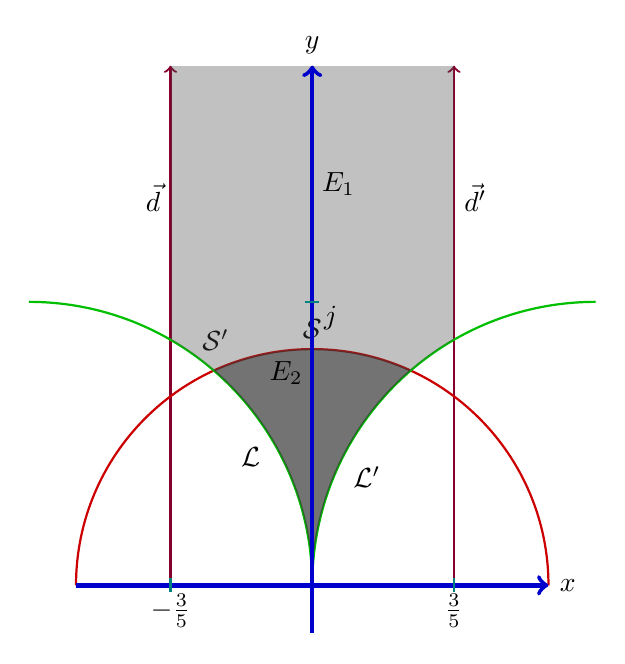
\begin{tikzpicture}[scale=3]
  \def\xmin{-1} \def\xmax{1}
  \def\ymin{-0.2} \def\ymax{2.2}

  % Axes
  \draw [ultra thick,->,color=blue!80!black] (\xmin,0) -- (\xmax,0) node[right,black] {$x$};
  \draw [ultra thick,->,color=blue!80!black] (0,\ymin) -- (0,\ymax) node[above,black] {$y$};

  % Tick marks
  \draw [thick,color=teal] (-0.6,-0.03) -- (-0.6,0.03) node [below=2,black] {$-\frac{3}{5}$};
  \draw [thick,color=teal] (0.6,-0.03) -- (0.6,0.03) node [below=2,black] {$\frac{3}{5}$};
  \draw [thick,color=teal] (-0.03,1.2) -- (0.03,1.2) node [below right=-2,black] {$j$};

  % Physics-related focus points
  \node at (0,1.7) [right,black] {$E_1$};
  \node at (0,0.9) [left,black] {$E_2$};

  \begin{pgfonlayer}{background}
    % Vertical lines
    \draw [thick,->,color=purple!70!black] (-0.6,0) -- (-0.6,\ymax) node [pos=0.7,above left,black] {$\vec{d}$};
    \draw [thick,->,color=purple!70!black] (0.6,0) -- (0.6,\ymax) node [pos=0.7,above right,black] {$\vec{d}'$};

    % Main arcs (paths of charged particles, for example)
    \draw [thick,color=red!80!black] (1,0) arc (0:180:1) node [auto,swap,pos=0.50,black] {$\mathcal{S}$} node [auto,swap,pos=0.60,black] {$\mathcal{S}'$};

    % Secondary arcs (fields or equipotentials)
    \draw [thick,color=green!75!black] (0,0) arc (0:90:1.2) node [auto,pos=0.35,black] {$\mathcal{L}$};
    \draw [thick,color=green!75!black] (1.2,1.2) arc (90:180:1.2) node [auto,pos=0.70,black] {$\mathcal{L}'$};

    % Clipping region for shading
    \path[clip] (1.2,\ymax) -- (1.2,1.2) arc (90:180:1.2) -- (0,0) arc (0:90:1.2) -- (-1.2,\ymax) -- cycle;

    \begin{scope}
      \path[clip] (1.2,\ymax) -- (1.2,1.2) arc (90:180:1.2) -- (0,0) arc (0:90:1.2) -- (-1.2,\ymax) -- cycle;
      \fill[black!40!gray,opacity=0.35] (-0.6,0) rectangle (0.6,\ymax);
      \fill[black!60!gray,opacity=0.55] (1,0) arc (0:180:1);
    \end{scope}
  \end{pgfonlayer}
\end{tikzpicture}

\end{document}